\documentclass[11pt]{article}

\usepackage{authblk}
\usepackage{graphicx}
\usepackage{amsmath}
\usepackage{hyperref}
\usepackage[margin=1in]{geometry}

% Use symbol footnotes (*, †, ‡, …)
\renewcommand\thefootnote{\fnsymbol{footnote}}

% ------------------------------
% Title & Authors
% ------------------------------
\title{easytrack: A napari plugin for automated parameter tuning in cell tracking}

% Shared corresponding author symbol using a single \thanks{}
\author[1,2]{Tim Huygelen}
\author[3]{Alan Lowe}
\author[1,2,*]{Yanlan Mao}
\author[1,2,*]{Pablo Vicente-Munuera}

% Affiliations
\affil[1]{Laboratory for Molecular Cell Biology, University College London, London, United Kingdom}
\affil[2]{Institute for the Physics of Living Systems, University College London, London, United Kingdom}
\affil[3]{Chan Zuckerberg Initiative, Redwood City, CA, USA}
\affil[*]{Corresponding authors: y.mao@ucl.ac.uk, p.munuera@ucl.ac.uk}

\begin{document}
\maketitle

\section*{Summary}
Life is in constant movement, even microscopic bodies like cells. To understand cellular dynamics, or how cells move and 
interact, we analyse time-lapse microscopy images that highlight cellular structures like membranes and nuclei. The 
bioimage community has developed automated tracking algorithms to follow cells over time and space, but these tools 
often require extensive manual parameter tuning and technical expertise. \texttt{easytrack} democratises cell tracking by 
providing an intuitive graphical interface and automating the parameter optimisation process, making these powerful 
algorithms accessible to researchers without computational backgrounds.

\section*{Statement of need}
Cell tracking, the process of following individual cells through time and space, is essential for quantifying dynamic 
cellular behaviours such as migration, division, and morphological changes. These measurements underpin research into 
tissue healing \cite{Tetley:2019}, developmental biology \cite{Valon:2021}, and cancer progression \cite{Hong:2016}. Despite 
advances in computational methods \cite{Ulman:2017, Maska:2023}, many tracking algorithms require careful tuning of 
multiple parameters to achieve accurate results \cite{Loffler:2021, Chenouard:2014}.

The lack of accessible parameter tuning tools creates a barrier between technological capability and practical 
application. Researchers often resort to default parameters or limited manual exploration of the parameter space, 
potentially missing optimal configurations for their specific datasets. While hyperparameter optimisation frameworks 
like Optuna \cite{Optuna:2019} have proven effective in machine learning contexts, their application to cell tracking 
software remains limited, with no existing tools providing an accessible interface for biologists.

\texttt{easytrack} addresses this gap by implementing automated parameter tuning within the napari ecosystem \cite{napari:2019}, 
leveraging Bayesian optimisation techniques including Tree-structured Parzen Estimators (TPE) \cite{Ozaki:2022}. By 
automating what was previously a manual, iterative process, \texttt{easytrack} makes high-accuracy cell tracking accessible to 
researchers without computational expertise whilst reducing the time required from hours to minutes.

\section*{State of the field}
Cellular dynamics (how cells move, divide, and interact) are fundamental to understanding biological processes from 
tissue development to disease progression. Time-lapse microscopy enables researchers to capture these processes, but 
extracting quantitative information requires accurately tracking individual cells across image sequences. Current cell 
tracking software falls into two categories: general-use tools with modest accuracy, or high-performance algorithms like 
btrack \cite{btrack:2017, btrack:2021} that require extensive manual parameter tuning. This manual tuning is 
labour-intensive, requires expertise, and often needs repetition for different datasets or experimental conditions. 
For instance, for btrack, a Bayesian cell tracking algorithm, this involves configuring 18 parameters across its motion 
and hypothesis models. 
\texttt{easytrack} democratises access to high-accuracy cell tracking by automating the parameter optimisation process through 
a user-friendly napari plugin interface.

\section*{Software Design}
\texttt{easytrack} is implemented as \texttt{napari-easytrack}, a plugin for the napari multi-dimensional image viewer, integrating 
seamlessly with the growing napari bioimage analysis ecosystem. The design philosophy emphasises composability over 
reinvention, building upon established open-source tools: btrack for tracking \cite{btrack:2017, btrack:2021}, Optuna for 
optimisation \cite{Optuna:2019}, and traccuracy for evaluation \cite{Traccuracy:2023}.

\subsection*{Architecture}
The plugin provides two complementary widgets (Figure \ref{fig:workflow}): 
\begin{itemize}
\item {\textbf{Parameter tuning widget}:} Automates the process of finding optimal btrack parameters for given data using Bayesian 
optimisation. Users provide ground truth annotations (cells that have been segmented and tracked), and the widget 
optimises btrack's 18 parameters by minimising the difference between predicted and ground truth tracking. The 
optimisation can be performed using TPE (Tree-structured Parzen Estimator) and random search and evaluates tracking 
quality using the AOGM metric from the Cell Tracking Challenge \cite{Maska:2014}. Optimised parameters are saved as JSON 
configuration files for subsequent use. 
\item{\textbf{Tracking widget}:} Applies previously optimised or manually created parameter configurations to new segmented 
time-lapse or 3D images. The widget parses JSON configuration files, executes btrack with the specified parameters, and 
displays tracked cells with their trajectories overlaid for visual inspection and manual correction if needed. 
Both widgets include segmentation preprocessing functionality to remove small artefacts that can compromise tracking 
accuracy. 
\end{itemize}

\begin{figure}[h]
	\centering
	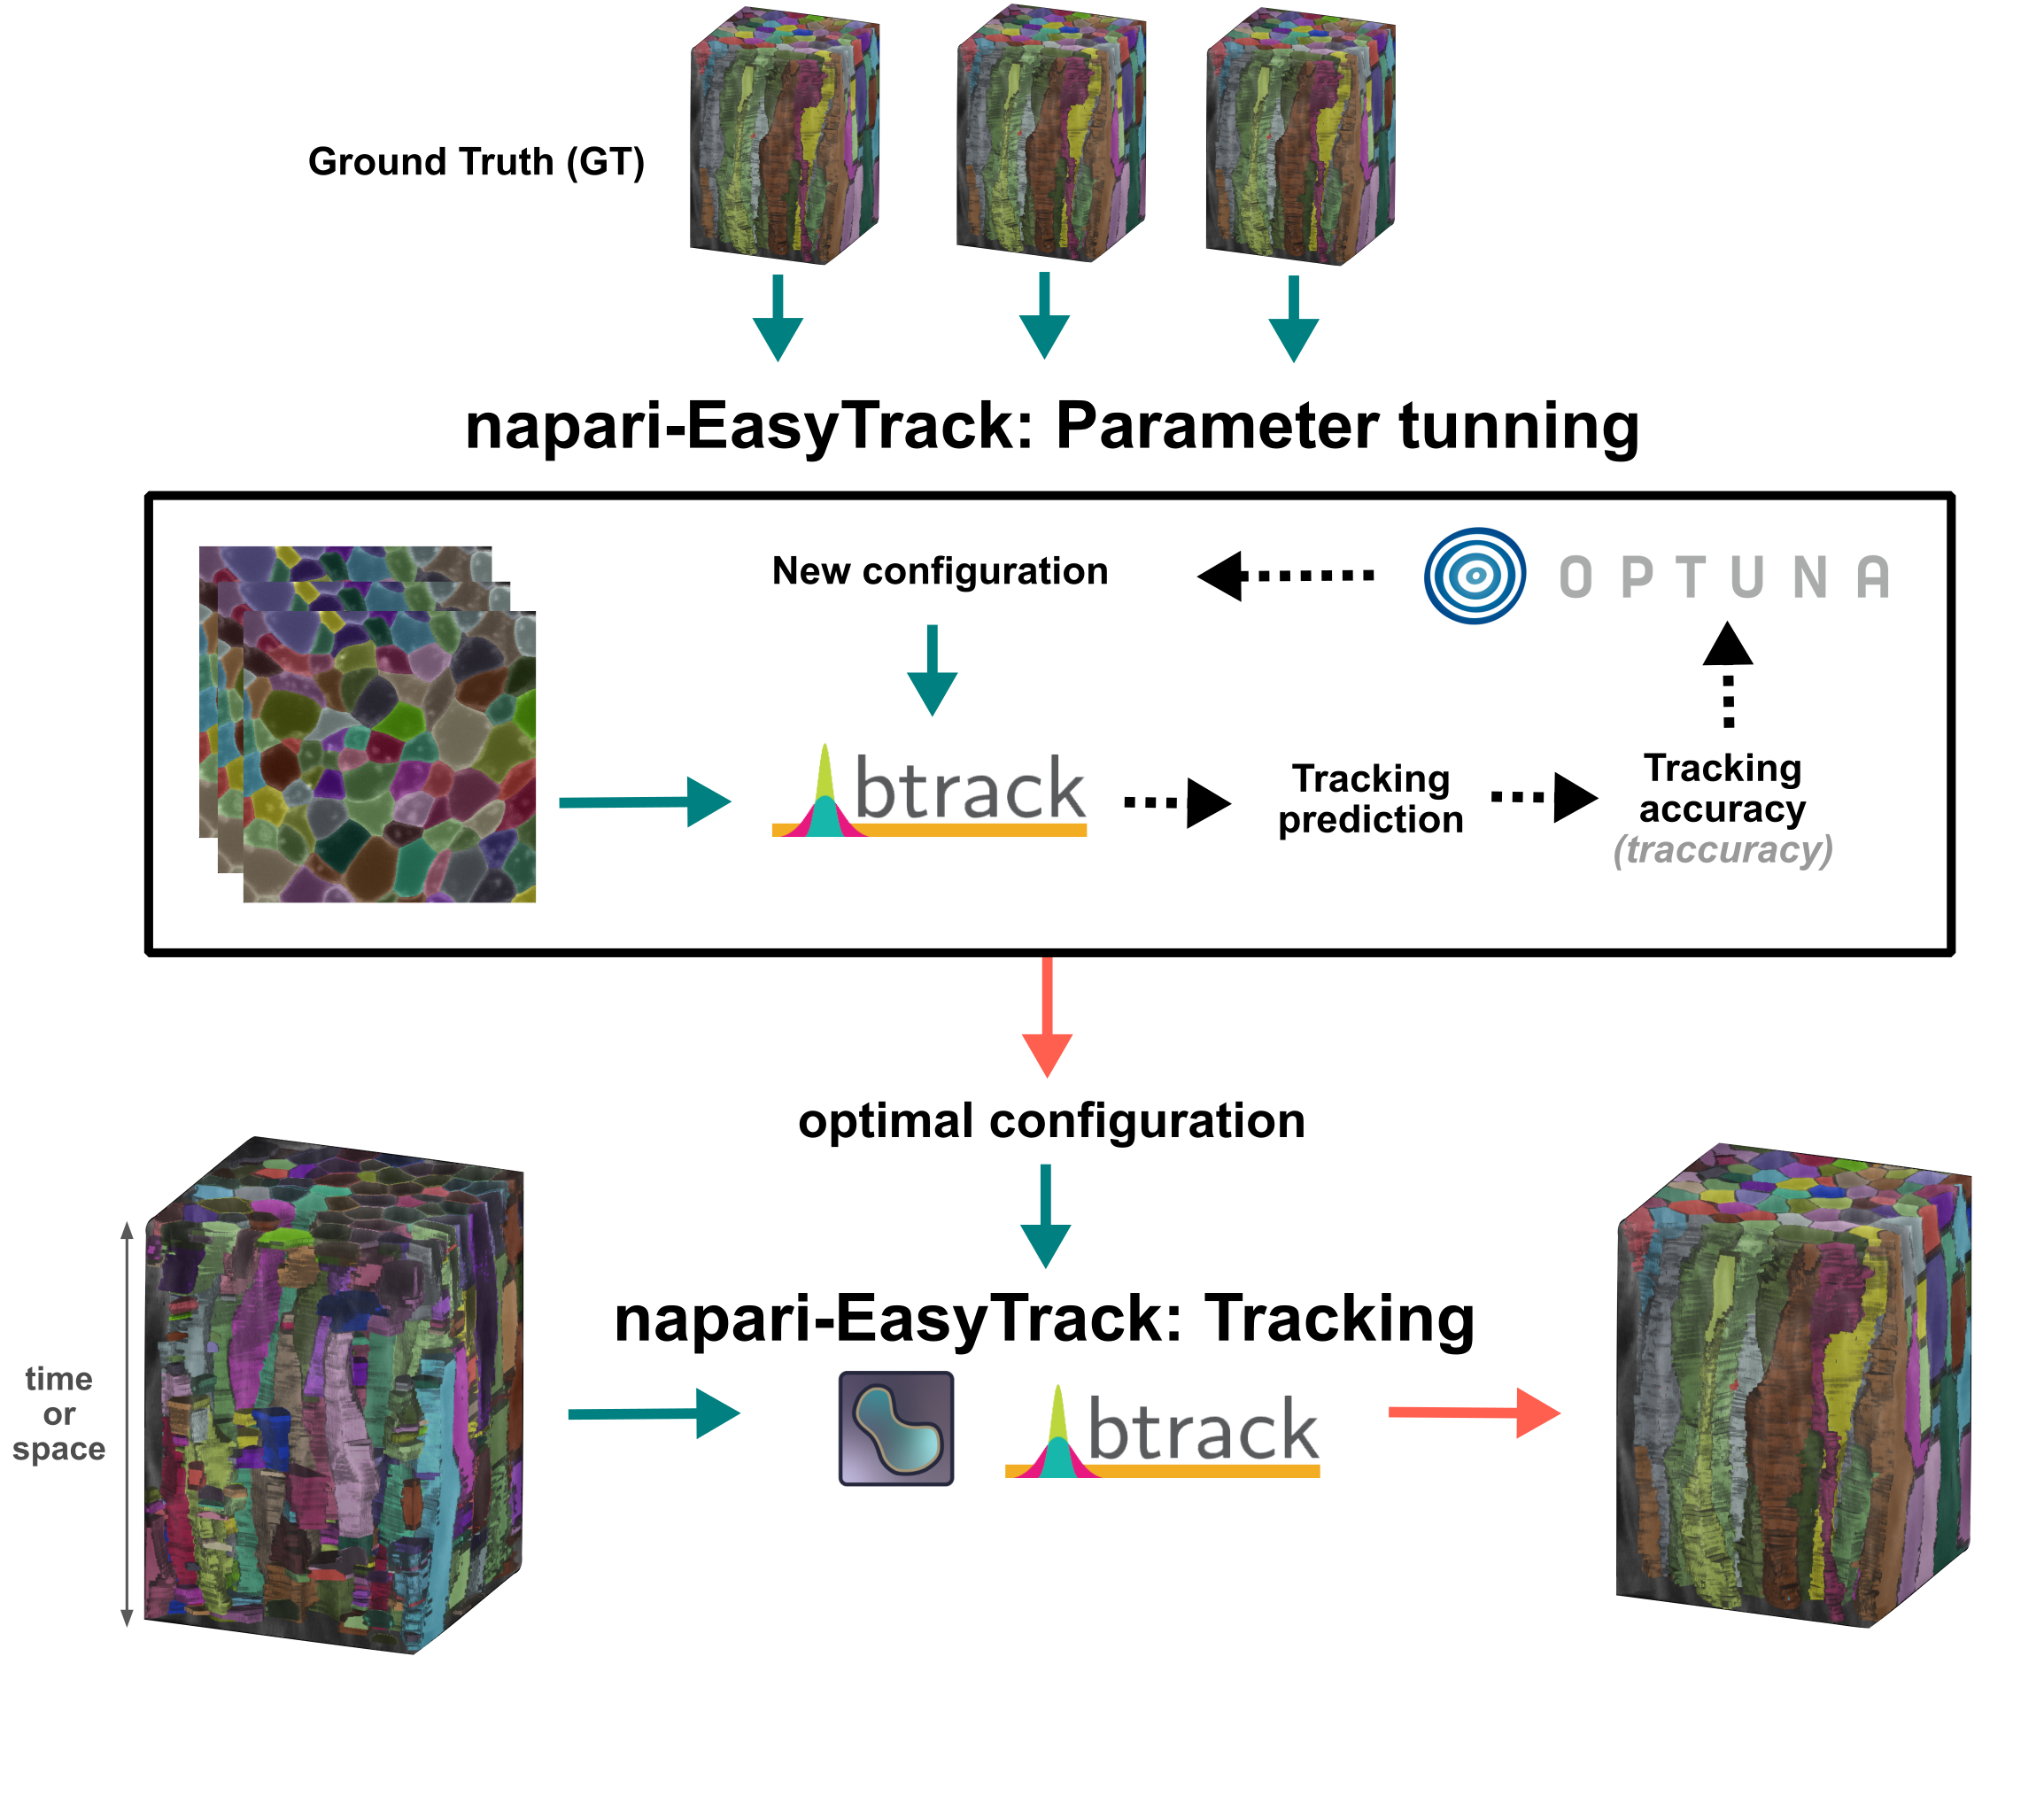
\includegraphics[width=\linewidth]{Fig_1_Workflow.png}
	\caption{Workflow of the napari plugin \texttt{easytrack}. 
		The parameter tuning widget (top) uses ground truth annotations to optimise btrack parameters via Bayesian optimisation, 
		Optuna and traccuracy for the optimisation process. 
		The tracking widget (bottom) applies these optimised parameters to new datasets.\label{fig:workflow}}
\end{figure}

\section*{Research impact statement}
Sophisticated cell tracking algorithms often remain underutilised due to their complexity \cite{Soelistyo:2023}. \texttt{easytrack} 
addresses this usability barrier by automating parameter tuning, enabling: 
\begin{enumerate}
	\item \textbf{Reproducible research:} Parameter configurations can be saved, shared, and reused, reducing variability across 
	studies. 
	\item \textbf{Efficiency gains:} Optimisation completes in tens of minutes compared to hours or days of manual tuning. 
	\item \textbf{Accessibility:} Non-experts can leverage state-of-the-art tracking without deep algorithmic knowledge. 
\end{enumerate}
In the age of artificial intelligence, there are many tools obtaining segmentation from microscopy 
images \cite{Cellpose:2021}. However, for complex 3D segmentations a tracking step is required to get an accurate 
result \cite{Paci:2025}. \texttt{easytrack} has already been integrated into napari-EpiTools \cite{EpiTools:2025}, a tool for analysing 
packed epithelial tissues that was previously missing a tracking algorithm with a simplified graphical user interface. 
This integration allows EpiTools' user base to benefit from automated parameter tuning for accurate 3D tracking. While 
btrack is one of the most popular and robust plugins in napari, it is not specialised for packed epithelial tissues. 
Therefore, even though \texttt{easytrack} is in its early stages, it fills a gap in the napari community for easy-to-use tracking tools, particularly for epithelial tissues and 3D stitching, whilst its implementation as a standalone plugin ensures broader accessibility across the napari community. 

\section*{AI usage policy}
GitHub Copilot and Claude were used to assist in writing portions of the code for this project. All code was reviewed, tested, and edited by the authors. 

\section*{Acknowledgements}
We thank the Mao laboratory for providing valuable feedback on the graphical user interface and thoroughly testing \texttt{easytrack} during development. We also acknowledge the napari and btrack communities for creating the foundational tools upon which this work builds. 

\bibliographystyle{plain}
\bibliography{paper}

\end{document}